\documentclass[12pt]{report}

%% limba document
\usepackage[romanian]{babel}
\selectlanguage{romanian}

%% font lucrare
\usepackage[utf8]{inputenc}
\usepackage[T1]{fontenc}
\usepackage{mathptmx}

%figuri
\usepackage{graphicx}
%braket
\usepackage{braket}
%% geometria paginii
\usepackage{geometry}
%% setari antet/subsol
\usepackage{fancyhdr}
%% indentare primul paragraf din capitol
\usepackage{indentfirst}
\usepackage[unicode, hidelinks, colorlinks, linkcolor=black, urlcolor=blue, citecolor=black]{hyperref}
%% culoare text (pe moment folosit in titluri de capitole)
%% https://www.overleaf.com/learn/latex/Using_colours_in_LaTeX
\usepackage[dvipsnames]{xcolor}
%% format titlu capitol/subcapitol/etc
\usepackage{titlesec}
%% titluri pentru figuri/tabele/listing-uri de cod/etc.
\usepackage{caption}
%% pozitionare float-uri (figuri/tabele/etc)
\usepackage{float}
%% pentru tabele pe mai multe pagini
\usepackage{longtable}	
%% pentru tabele cu celule cu mai multe linii
\usepackage{multirow}			
%% pentru ecuatii
\usepackage{amsmath}
%% pentru definitii, teoreme
\usepackage{amsthm}
%% pentru algoritmi, pachetul algorithm este cel mai basic
\usepackage[chapter]{algorithm}
\usepackage[noend]{algpseudocode}
% daca pachetul algorithm nu este satisfacator pentru ceea ce aveti de scris, mai exista pachetele:
% algorithmic, algorithmicx, algpseudocode, algorithm2e
% https://tex.stackexchange.com/questions/229355/algorithm-algorithmic-algorithmicx-algorithm2e-algpseudocode-confused
%% formatari listing
\usepackage{listings}
% https://www.overleaf.com/learn/latex/Code_listing
%% pachetul minted formateaza/coloreaza sintaxa codului sursa, spre deosebire de pachetul listings care doar face bold pe sintaxa
\usepackage[newfloat]{minted}
% https://www.overleaf.com/learn/latex/Code_Highlighting_with_minted


%% setup dimensiune pagina, dimensiune header/footer
%% setup dimensiune 16pt
%% valorile generice, pentru documentul in ansamblu
%% in mod uzual, nu ar trebui modificate

%% dimensiune pagina text, header/footer
\geometry{
    a4paper,
    left=2.5cm,
    right=2cm,
    top=2cm,
    bottom=2cm,
    headheight=0.55cm, %% daca am fi mers strict pe 0.5cm, am fi avut warning-uri
    footskip=0.55cm,
}

%% spatiere paragrafe si indentari
\linespread{1.0}                % spatierea intre randuri de 1 rand
\setlength{\parskip}{0pt}       % spatierea intre paragrafe
\setlength{\parindent}{1.27cm}  % identare paragraf de 1.27 cm

%% dimensiune font 16pt
\newcommand{\almostLarge}{\fontsize{16pt}{20pt}\selectfont}
%% date caracteristice universitatii/facultatii.
%% in acest fisier nu trebuie aduse modificari, cu exceptia tipului de teza si a anului in care este sustinuta teza
%% comune: coperta externa si interna
\newcommand{\university}    {UNIVERSITATEA TEHNICĂ „Gheorghe Asachi” din IAȘI}
\newcommand{\faculty}       {FACULTATEA DE AUTOMATICĂ ȘI CALCULATOARE}
\newcommand{\studyfieldlbl} {DOMENIUL: }
\newcommand{\studyfield}    {Calculatoare și Tehnologia Informației}
\newcommand{\studyproglbl}  {SPECIALIZAREA: }
\newcommand{\studyprog}     {Tehnologia Informației}
\newcommand{\promotion}     {2022}
\newcommand{\location}      {Iași}

%% absolventii de master vor inlocui "diploma" cu "disertatie"
\newcommand{\thesistype}    {Lucrare de diplomă}
%\newcommand{\thesistype}    {Lucrare de disertație}
%% datele specifice: nume, prenume student; titlu lucrare; nume, prenume, grad didactic coordonator
%% PENTRU MODIFICARE SE EDITEAZA FISIERUL macros/student.tex
%% date student si lucrare
\newcommand{\thesistitle}   {Analiză comparativă a metodelor clasice și cuantice
de generare a numerelor aleatoare. Aplicație.}    %<---------
\newcommand{\authorlast}    {Stoian}         %<---------
\newcommand{\authorfirst}   {Alin-Bogdan}
\newcommand{\authornamefl}  {\authorfirst \space \authorlast} % first name last
\newcommand{\authornamelf}  {\authorlast \space \authorfirst} % last name first

%% titlul academic si numele coordonatorului stiintific
\newcommand{\coordinator}   {Ș.l. dr. ing. Petrilă Iosif-Iulian}
%% pentru numele complet si grad didactic/titlu academic, consultati https://ac.tuiasi.ro/despre/personal/cadre-didactice-ale-departamentului-de-calculatoare/



\usepackage[nottoc]{tocbibind}
\usepackage[unicode, hidelinks, colorlinks, linkcolor=black, urlcolor=blue, citecolor=black]{hyperref}

\begin{document}
\sloppy

%% definitii culori
\definecolor{albastru-ac}{HTML}{004586}

\titleformat
    {\chapter}
    [hang]
    {\color{albastru-ac}\bfseries\large}
    {}
    {0pt}
    {}
    []
    
\titlespacing
    {\chapter}%
    {1.27cm}
    {0.42cm}
    {0.21cm}
    [0pt]

\titleformat
    {\section}
    [hang]
    {\color{albastru-ac}\bfseries\large}
    {}
    {0pt}
    {}
    []
    
\titlespacing
    {\section}%
    {1.27cm}
    {0.42cm}
    {0.21cm}
    [0pt]

\begin{center}
    \large
    {\textbf{\thesistype} -- \textbf{Raport nr. 2}}
    
    \vspace{0.5cm}
    
    \normalsize
    \textbf{\thesistitle}
\end{center}

\textit{Student}: \textbf{\authornamelf}

\textit{Coordonator științific}: \textbf{\coordinator}

\vspace{0.5cm}
\iffalse
Al doilea raport trebuie să aibă minim 5-6 pagini și să conțină:

\section*{Proiectarea hardware/software a aplicației}

La data la care ar trebui predat acest raport, aplicația proiectului de licență ar trebui să fie în stadiul în care proiectarea este finalizată, implementarea se află într-un stadiu avansat și ar trebui să fi fost realizate primele experimente și să fi obținut un set primar de rezultate experimentale.

În acest capitol va fi descrisă, pe scurt, arhitectura aplicației, modele/diagrame (elemente specifice Capitolului 2 din documentația lucrării de licență), precum și modul în care au ajuns să fie implementate (elemente specifice Capitolului 3).

În acest capitol nu trebuie furnizate amănunte, având rolul descrierii soluției tehnice de ansamblu.

\section*{Rezultate intermediare obținute}

Primele rezultate ar trebui să confirme soluția aleasă și să se încadreze, cu o marjă, în rezultatele așteptate descrise în primul raport intermediar.

Dacă sunt obținute anomalii, acestea ar trebui să aibă o explicație/justificare care ar trebui introdusă în acest capitol, eventual soluții de rafinare a rezultatelor care ar putea fi aplicate în timpul rămas până la predarea lucrării.

\section*{Dificultății/provocări întâmpinate și soluții de rezolvare}

În această secțiune pot fi incluse elementele corespunzătoare din capitolul al treilea al tezei.

Acest capitol nu trebuie să includă dificultăți din categoria „nu am găsit pe net soluția”, „mi-a fost greu să mă adaptez cu limbajul de programare ales” sau „resurse hardware insuficiente”.

Acest capitol ar putea fi organizat și sub forma Problemă întâmpinată / Soluție aleasă.
Ideal ar fi să fi identificat mai multe soluții posibile și ați ales, justificat, una dintre acestea pe baza unor argumente care țin de specificul temei alese, natura datelor prelucrate etc.
\fi

\section*{Proiectarea hardware/software a aplicației}

În momentul scrierii acestui raport, majoritatea funcționalității de bază pentru aplicația de generare de numere și testarea lor este completă, inclusiv partea de execuție pe un calculator cuantic adevărat, pe Cloud (voi detalia mai târziu). Totuși, cum această aplicație (nu e cea cu interfață utilizator pe care o menționez în titlu) este sub forma unui Jupyter Notebook și un script Python separat, nu se poate discuta despre o anumită "proiectare" a vreunei aplicații. Voi prezenta, totuși, circuitele cuantice utilizate și voi detalia asptectele calculatorului cuantic pe care am executat codul meu, dar și metoda de interfațare cu acesta.

\subsection*{Elemente hardware}

Cum scopul lucrării este măsurarea de performanțe comparativ între mai multe metode de generare de numere aleatoare, din care unele sunt bazate strict pe simulare și executare pe calculatoare clasice, voi enumera aici componentele și sistemele de operare utilizate pe calculatoarele pe care am rulat metodele prezentate. Desigur, cum analiza este comparativă, nu contează foarte mult valorile absolute, ci cum sunt ele relativ față de celelalte.

\vspace{0.5cm}
\textbf{Laptop I} - Lenovo - Y520
\begin{itemize}
    \item Laptop cu sistemul de operare Windows
    \item 8 GB RAM
    \item CPU Intel i7-7700HQ @ 2.8 GHz, 8 cores
    \item GPU NVidia GeForce GTX 1060 8 GB VRAM, 4 Shared RAM
    \item HDD 1 TB
\end{itemize}

\vspace{0.5cm}
\textbf{Laptop II}  - Myria - MY8312SV
\begin{itemize}
    \item Laptop cu sistemul de operare Linux - Xubuntu
    \item 4 GB RAM
    \item CPU Intel Pentium N4200 @ 2.5 GHz, 4 cores
    \item GPU Intel HD Graphics 505
    \item SSD 256 GB
\end{itemize}

Calculatorul cuantic utilizat în executarea experimentelor este "ibmq\_bogota", un calculator cuantic dezvoltat și menținut de către IBM Labs, cu care voi interfața printr-un API Cloud, despre care voi discuta în secțiunea "software". Specificațiile calculatorului cuantic sunt următoarele:
\begin{itemize}
    \item 5 Qubiți
    \item 32 Volum Cuantic
    \item 2.3K CLOPS
    \item Tip de procesor: Falcon r4L
    \item Version: 1.6.37
    \item Basis gates: CX, ID, RZ, SX, X
\end{itemize}

Explicațiile specificațiilor sunt următoarele:
\begin{itemize}
    \item Qubiți - Cantitatea de qubiți pe care o are disponibilă calculatorul cuantic; aceștia au o anumită configurație prezentă în figura \ref{fig:TopologieBogota}. Qubiții legați unii de ceilalți pot fi entangled sau se pot executa porți logice cuantice pe mai mulți qubiți între ei, fără a putea face acest lucru între qubiți care nu au conexiune între ei. Conexiunea este fizică și legată strict de design-ul calculatorului cuantic.
    \item Volum Cuantic - O unitate de măsură care reprezintă "dimensiunea" maximă a unui circuit cuantic care poate fi executat de un calculator cuantic. De exemplu, dacă un calculator cuantic cu 8 qubiți poate executa un circuit în care se vor afla maxim 8 stări $\ket{\psi}$ intermediare, atunci spunem că acel calculator are un Volum Cuantic de 256. Prin urmare, volumul cuantic este o specificație de performanță independentă de hardware-ul abstractizat.
    \item CLOPS - Circuit Layer Operations Per Second - Câte straturi de volum cuantic pot fi executate de un QPU (Quantum Processing Unit) într-o unitate de timp. Documentația de la IBM \cite{misc:web:DocumentatieIBMQ} recomandă lectura lucrării \cite{misc:paper:QSS:WackAndrewEtAl} pentru a înțelege conceptul mai bine.
    \item Tipul de procesor: Există o mare varietate de QPU-uri dezvoltate, atât de către IBM, cât și de către alte firme. Familia de procesoare \textit{Falcon} cu seria r4 sunt o platformă pentru circuite de medii dimensiuni, iar calculatorul IBMQ\_Bogota este unul disponibil public, gratuit, prin API-ul cloud de la IBM Quantum Cloud.
    \item Versiunea: versiunea procesorului în ansamblu.
    \item Basis gates: porțile compatibile cu QPU-ul dat. Orice circuit care folosește alte porți trebuie \textit{transpilat}, adică trebuiesc descompuse toate celelalte porți în aceste porți pentru a putea fi executat. Qiskit, framework-ul pentru calcul cuantic de la IBM, permite transpilarea automată a oricăror circuite în circuite compatibile cu calculatoarele cuantice disponibile public.
\end{itemize}

\begin{figure}[H]
    \centering
    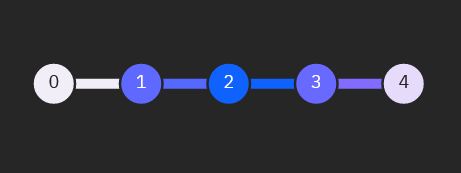
\includegraphics{anexe/figuri/TopologieBogota.png}
    \caption{Topologia fizică a calculatorului cuantic \textit{IBMQ\_Bogota} }
    \label{fig:TopologieBogota}
\end{figure}
\pagebreak
\subsection*{Elemente Software}

Cum am mai spus, în momentul de față doar aplicația pentru design-ul circuitelor și a testării corectitudinii generării de numere aleatoare, împreună cu câteva elemente de măsură de performanță sunt realizate. Cum acestea sunt făcute sub forma unui Jupyter Notebook, respectiv a unui script Python, nu se poate pune problema unei "proiectări" propriu-zise a vreunei aplicații. Voi prezenta totuși circuitele realizate de mine și cele luate gata făcute din bibliotecile Qiskit\_finance, framework despre care am discutat în raportul precedent.

\vspace{0.5cm}
\textbf{Cel mai simplu circuit}
\begin{figure}[H]
    \centering
    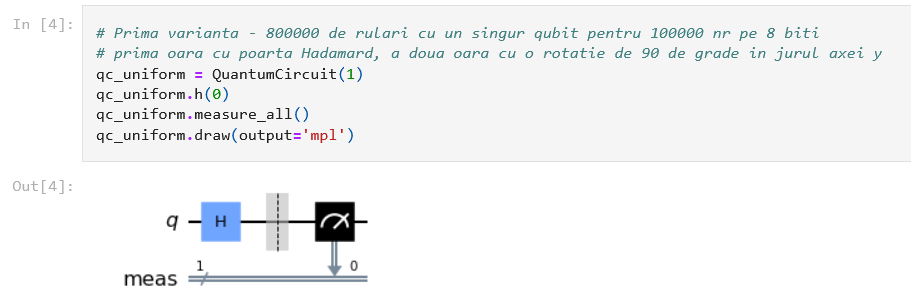
\includegraphics[scale=0.80]{anexe/figuri/CircuitHadamard1.png}
    \caption{Un circuit simplu, cu o singură poartă Hadamard, cu scopul de a genera numere pe 8 biți, pe o distribuție uniformă, bit cu bit}
    \label{fig:CircuitHadamard1}
\end{figure}

\textbf{Variație pentru primul circuit}
\begin{figure}[H]
    \centering
    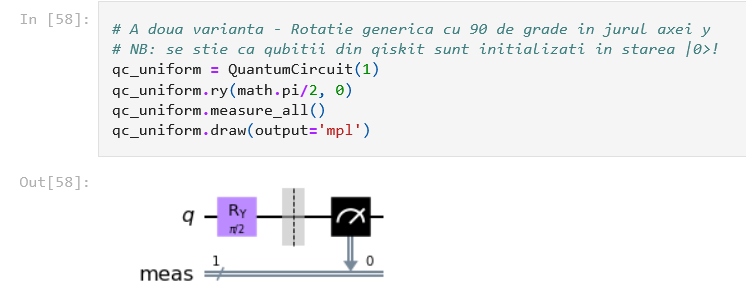
\includegraphics[scale=0.80]{anexe/figuri/CircuitRy1.png}
    \caption{Aceeași logică ca și pentru primul circuit}
    \label{fig:CircuitRy1}
\end{figure}

\textbf{Variante cu 8 qubiți pentru primele circuite} - Generază numerele imediat, fără a mai fi nevoie de concatenare, dar folosesc mai mulți qubiți și necesită mai multă executare la nivel fizic.

\begin{figure}[H]
    \centering
    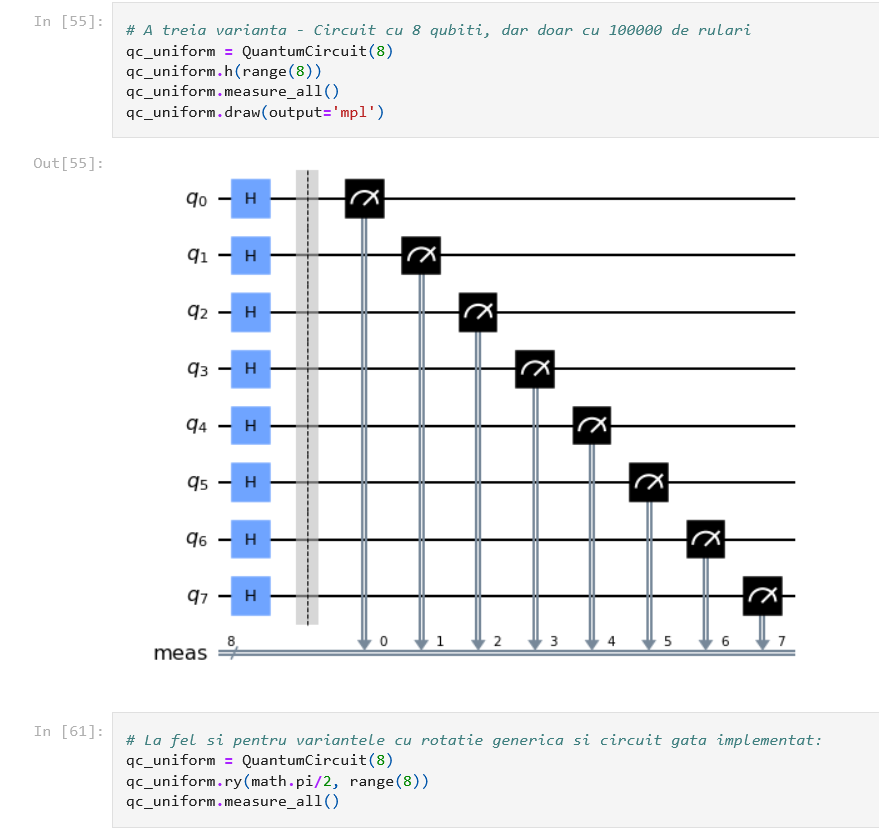
\includegraphics[scale=0.80]{anexe/figuri/Variante8Qubiti.png}
    \caption{Varianta cu 8 qubiți}
    \label{fig:Varianta8Qubiti}
\end{figure}

\textbf{Circuitul pentru distribuție uniformă} - De menționat că folosesc modului Initialize din Qiskit, dându-i ca argument radicalul unei distribuții normale pseudoaleatoare generată cu scipy.stats.multivariate\_normal.pdf(), normalizată. Așadar, nu știu cum se realizează circuitul la nivelul porților logice, framework-ul ocupându-se de modelarea acestuia și pretarea pe probabilitățile date de mine!

\begin{figure}[H]
    \centering
    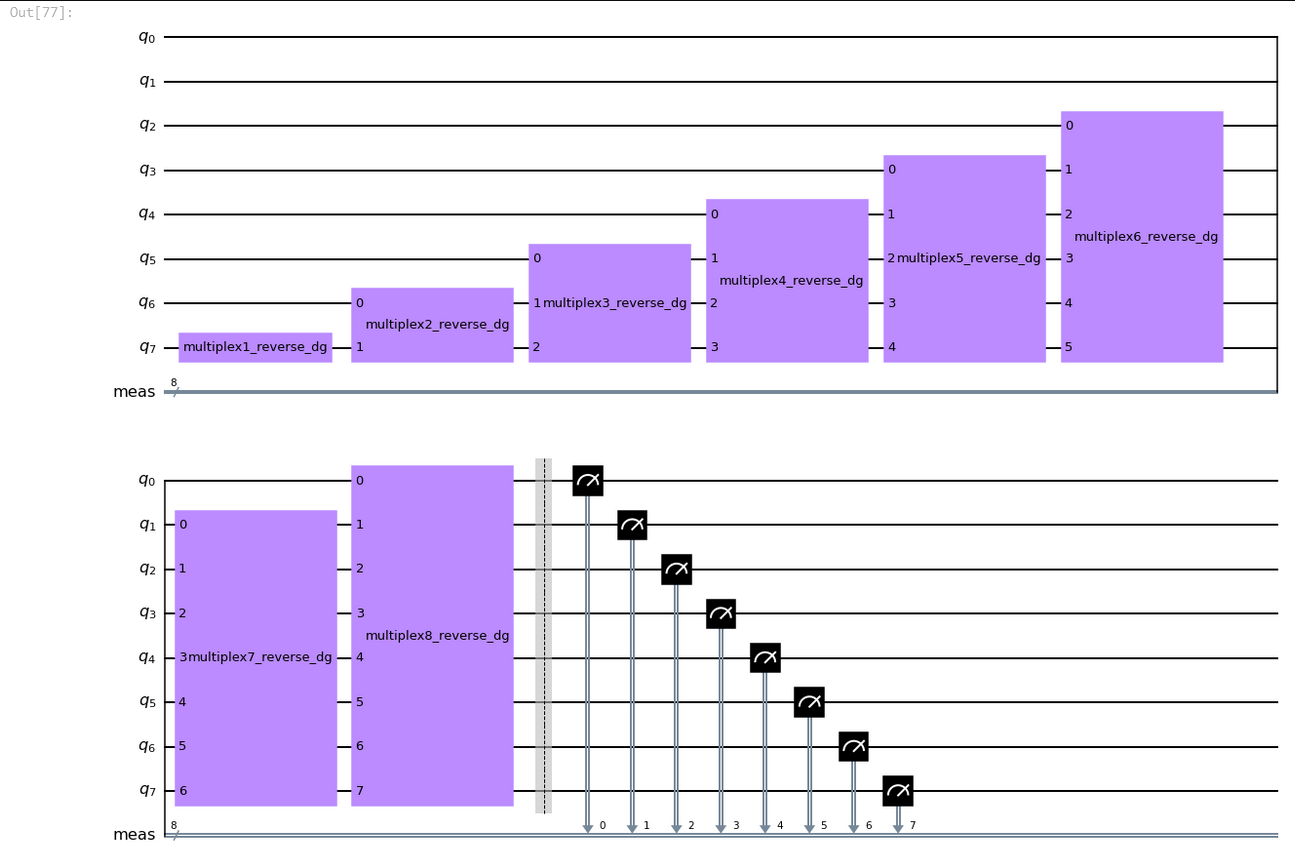
\includegraphics[scale=0.6]{anexe/figuri/CircuitNormalEu.png}
    \caption{Circuitul asamblat de Initialize(), cu module de porți logice}
    \label{fig:CircuitNormalEu}
\end{figure}
\pagebreak
\subsection*{Rezultate intermediare}
Toate circuitele prezentate au fost executate prin simulare, dar numai unele au fost executate și pe un calculator cuantic adevărat. Am realizat și verificarea aleatorității folosind teste statistice, și am și unele măsurători de performanță. Acestea sunt:

\textbf{Circuit uniform, 8 biți, porți Hadamard} - dataframe asociat rezultatelor și vizualizarea distribuției

\begin{figure}[H]
    \centering
    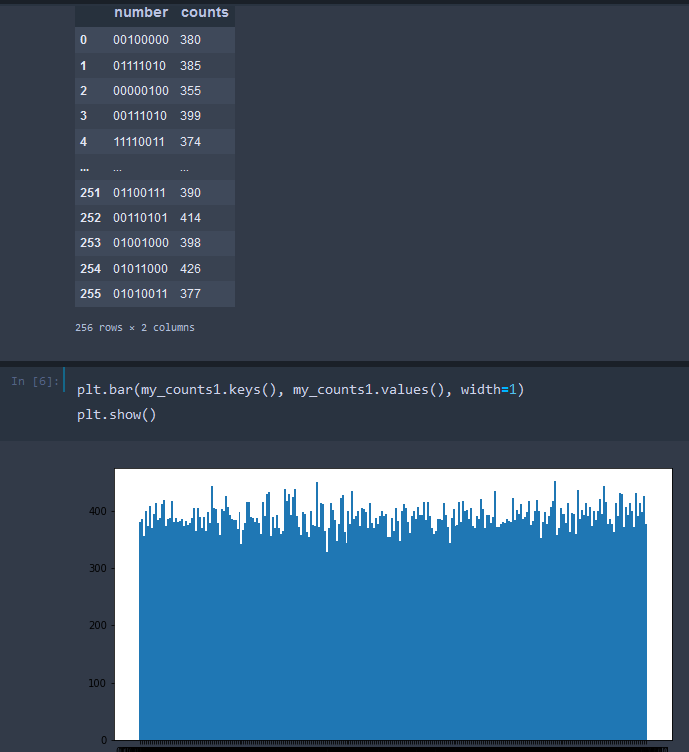
\includegraphics[scale=0.8]{anexe/figuri/Uniform8BitiEu.png}
    \caption{}
    \label{fig:Uniform8BitiEu}
\end{figure}

\textbf{Rezultat test statistic}

\begin{figure}[H]
    \centering
    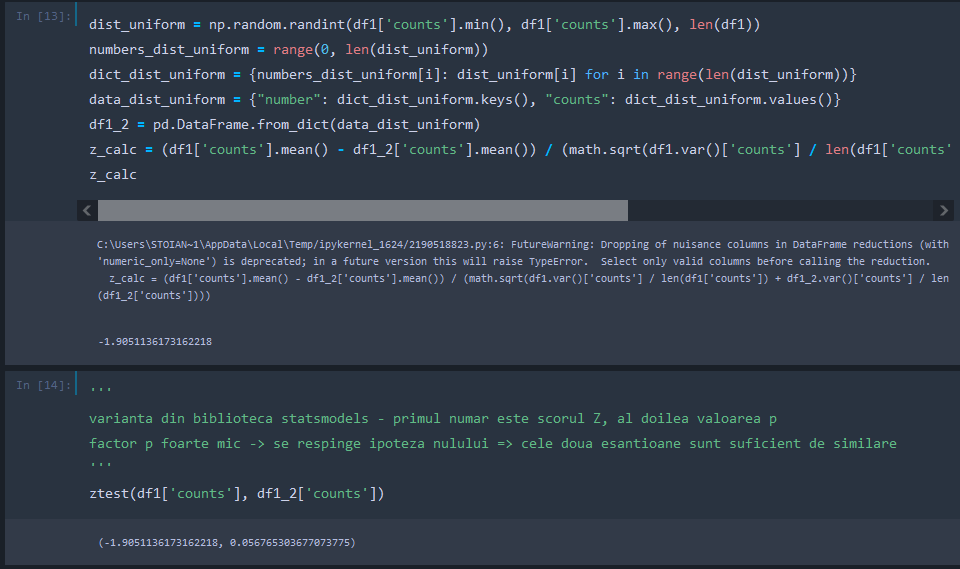
\includegraphics[scale=0.8]{anexe/figuri/TestZ8bitiHadamard.png}
    \caption{}
    \label{fig:TestZ8BitiHadamard}
\end{figure}
Rezultatele sunt < z critic, cu un factor p suficient de mic pentru a respinge ipoteza nulului ("distribuția dată nu are aceeași distribuție cu o distribuție știută drept uniformă")

\textbf{Circuit normal, 8 biți, inițializat de mine} - dataframe asociat rezultatelor și vizualizarea distribuției

\begin{figure}[H]
    \centering
    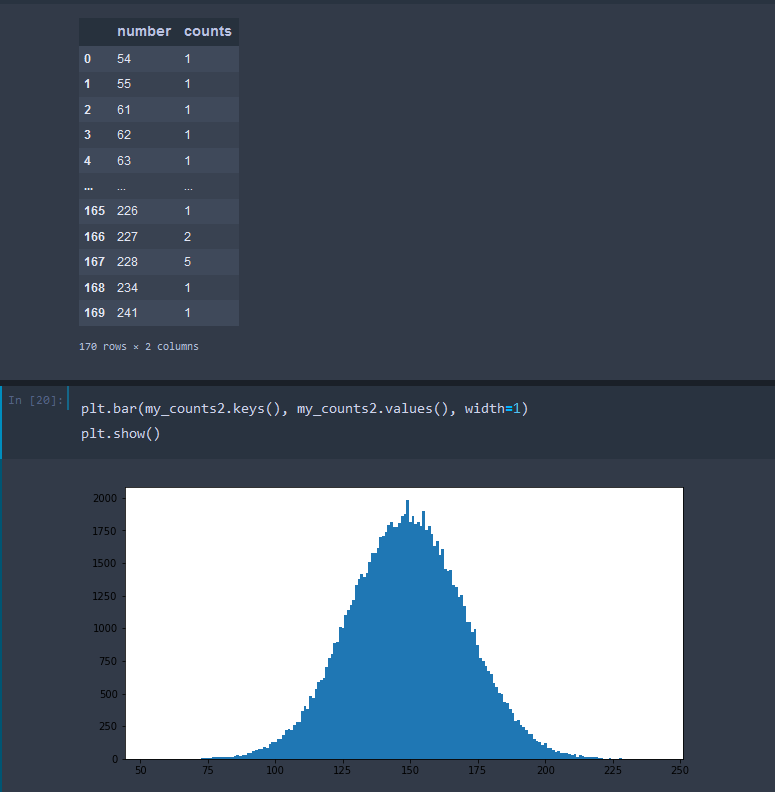
\includegraphics{anexe/figuri/Normal8BitiEu.png}
    \caption{}
    \label{fig:RezultatNormal8BitiEu}
\end{figure}




% *************** referinte bibliografice ***************
\nopagebreak
\bibliographystyle{IEEEtran}
\bibliography{bibliografie/bibliografie}

\end{document}